\section{Data}

\subsection{Description}
The data used for clustering were drawn from the back office system of a travel agency in Parga, Greece. The majority of the data are about hotel reservations. The rest are about excursions and transfers. The back office uses a relational database that contains x tables. After thoroughly examining the available data, only a few of them were kept for the analysis, the ones that seemed to have the most analytical value. Their relationships are shown in the following simplified diagram. \\
\begin{figure}[ht]
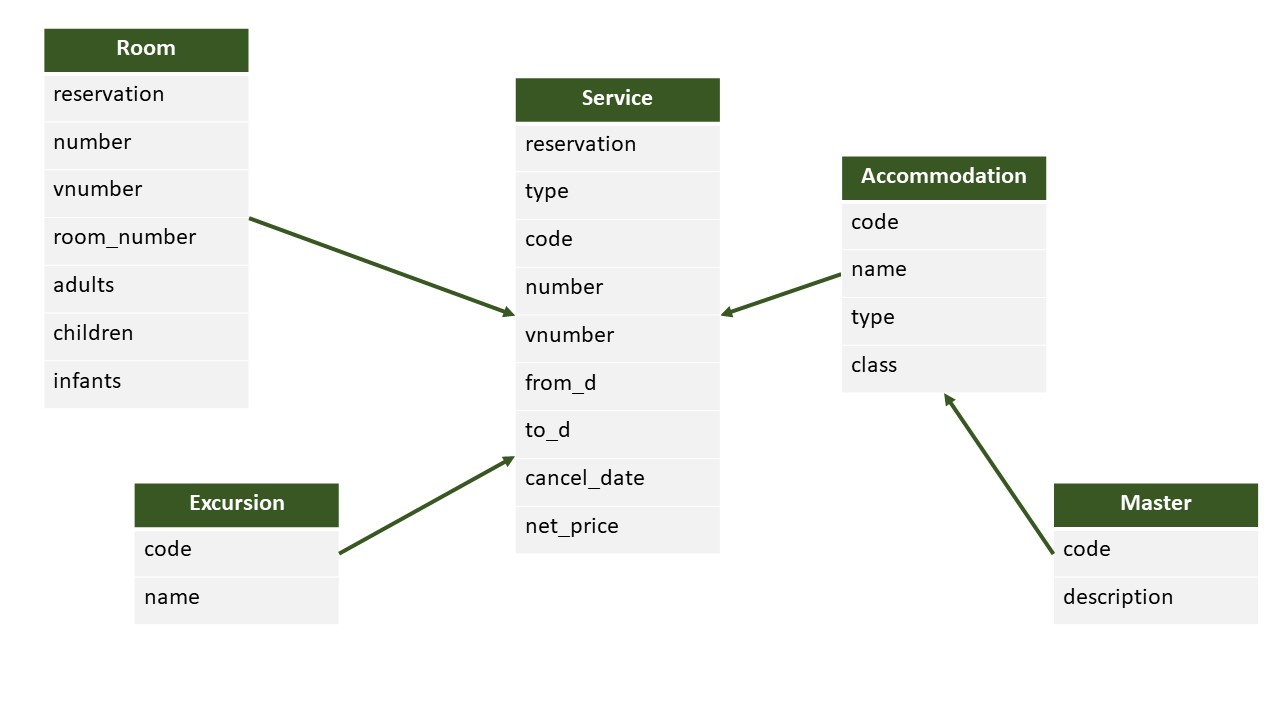
\includegraphics[width=\textwidth]{erp}
\caption{ERP diagram.}
\label{fig:erp}
\end{figure}
\\
One reservation may consist of many services (e.g., hotel reservation, excursion activity). For each service booked, there is at least one corresponding row on the 'Service' table that contains its details in a total of sixty-seven columns. Eleven of them were used and are explained in table \ref{tab:service}. \\
\begin{table}[h!]
\begin{center}
\begin{tabular}{l | p{12cm}}
\hline\hline
\textbf{Column} & \textbf{Description}\\
\hline\hline
reservation & Service's reservation identifier.\\
\hline
type & Service type. Can be either hotel(HTL), excursion(EXC) or transfer(TRF).\\
\hline
code & Service code from either 'Excursion', 'Hotel', or 'Transfer' tables.\\
\hline
number & Service number. The service's identifier number per reservation.\\
\hline
vnumber & Service vnumber. A number starting from one for each service per reservation. Whenever the service is edited a new row is created with the updated details and vnumber incremented by one.\\
\hline
fromd & Service's starting date.\\
\hline
tod & Service's ending date.\\
\hline
cancel\_date & The date the service booking gets canceled, in case it does.\\
\hline
net\_price & The total price of the booked service.\\
\hline
status & Reservation status. Can be either canceled(CL) or confirmed(CF). \\
\hline
customer\_id & Customer's identifier.\\
\hline\hline
\end{tabular}
\caption{Service table.}
\label{tab:service}
\end{center}
\end{table}
\\
Whenever an accommodation service is booked, the "Accommodation"(\ref{tab:accommodation}) table, holds the information that describes it. Using the service code set on the "Service" table the corresponding accommodation can be found. \\
\begin{table}[h!]
\begin{center}
\begin{tabular}{l | p{12cm}}
\hline\hline
\textbf{Column} & \textbf{Description}\\
\hline\hline
code & Accommodation identifier.\\
\hline
name & Accommodation name.\\
\hline
type & Accommodation type identifier. Categorical value that shows the type of the accommodation. \\
\hline
class & Accommodation class identifier. Categorical value that shows the quality of the accommodation. \\
\hline\hline
\end{tabular}
\caption{Accommodation table.}
\label{tab:accommodation}
\end{center}
\end{table}
\\
The "Master"(\ref{tab:master}) table contains several codes, and its descriptions, that can be found on many tables of the database, including the accommodation class and type codes. \\
\begin{table}[h!]
\begin{center}
\begin{tabular}{l | p{12cm}}
\hline\hline
\textbf{Column} & \textbf{Description}\\
\hline\hline
code & A code.\\
\hline
description & Code's description.\\
\hline\hline
\end{tabular}
\caption{Master table.}
\label{tab:master}
\end{center}
\end{table}
\\
Furthermore, whenever an accommodation is booked, at least one new row is entered in 'Room' table. These rows contain the information of the booked rooms of the accommodation, as described in table \ref{tab:room}. \\
\begin{table}[h!]
\begin{center}
\begin{tabular}{l | p{12cm}}
\hline\hline
\textbf{Column} & \textbf{Description}\\
\hline\hline
reservation & Service's reservation identifier.\\
\hline
number & Service number. The service's identifier number per reservation.\\
\hline
vnumber & Service vnumber. A number starting from one for each service per reservation. Whenever the service is edited a new row is created with the updated details and vnumber incremented by one.\\
\hline
room\_number & The number of rooms contained in this service booking with this specific composition.\\
\hline
adults & The number of adults in this room.\\
\hline
children & The number of children in this room.\\
\hline
infants & The number of infants in this room.\\
\hline\hline
\end{tabular}
\caption{Room table.}
\label{tab:room}
\end{center}
\end{table}
\\
Similarly to an accommodation booking, when an excurision is booked its details can be found through the service code of "Service" table in table \ref{tab:excursion}. \\
\begin{table}[h!]
\begin{center}
\begin{tabular}{l | p{12cm}}
\hline\hline
\textbf{Column} & \textbf{Description}\\
\hline\hline
code & Excursion identifier.\\
\hline
name & Excursion name.\\
\hline\hline
\end{tabular}
\caption{Excursion table.}
\label{tab:excursion}
\end{center}
\end{table}
\\
\subsection{Meta data extraction and reforming}
\section{Kmeans}
\section{Agglomerative Clustering}
